
\begin{frame}\frametitle{Solving the BSE}
  We rewrite the decomposition as
  \small\begin{equation}
  \!\!\!\!\!\!\!	\Gamma^\mu(k, Q)=\sum_{j=1}^{12} F_j(k^2, \omega, Q^2)it^\mu_j(k,Q), \quad F_j\in\{g_j,f_j\}, \; t^\mu\in\{G^\mu_j, T^\mu_j\}
  \end{equation}

  $$\!\!\!\!\!\!\!\!\!H_{ij}(k^2, \omega, Q^2)=1/4\mbox{Tr}\left\{\bar{t}^\mu_i(k,Q)t^\mu_j(k,Q)\right\}\neq\delta_{ij}\Longrightarrow t^\mu_j  \mbox{ not ortonormal }$$
  We want to construc an orthonormal basis $H_{ij}=\delta_{ij}$
  Fisrt we choose a frame for the four vectors:
  \begin{figure}[!htb]
  	\minipage{0.32\textwidth}
  	\hspace{-7mm}
  	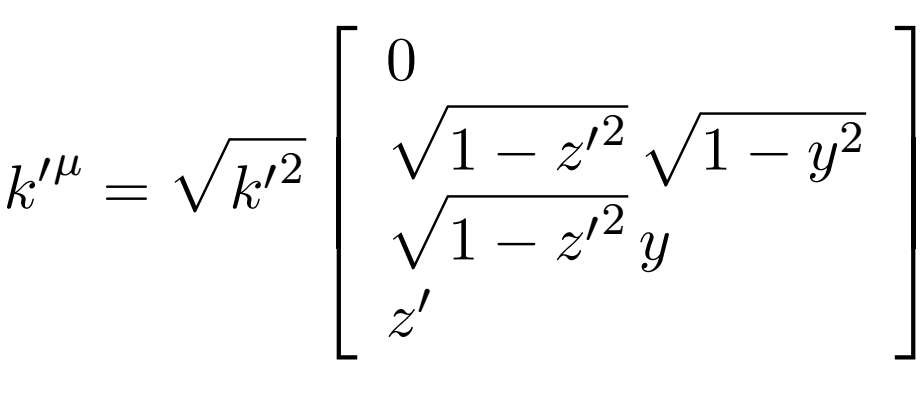
\includegraphics[width=4cm, height=2cm]{kps.png}

  	\endminipage\hfill
  	\minipage{0.32\textwidth}
  	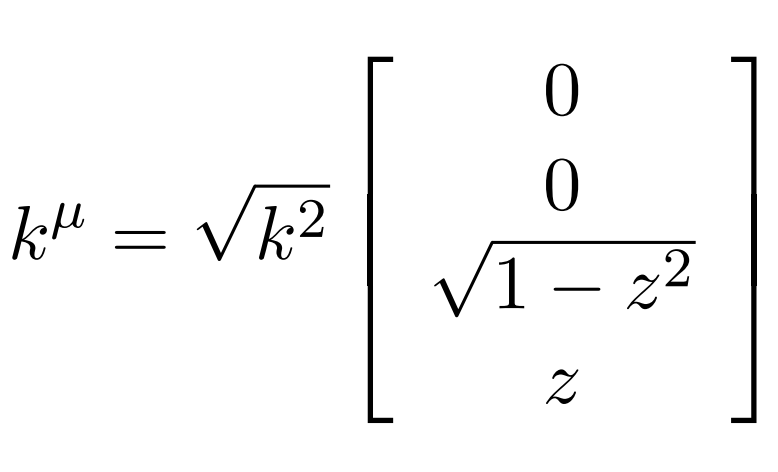
\includegraphics[width=\linewidth]{ks.png}

  	\endminipage\hfill
  	\minipage{0.32\textwidth}%
  	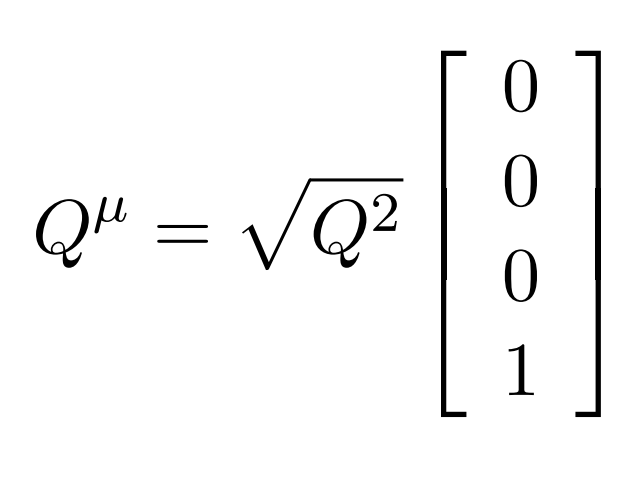
\includegraphics[width=\linewidth,  height=2.3cm]{Qs.png}

  	\endminipage
  \end{figure}
\end{frame}

\begin{frame}
	In this way we can express the quark-photon vertex in the following basis:
	\begin{equation}
		\Gamma^\mu(k, Q)=\sum_{j=1}^{12}a_(k^2, \omega, Q^2)i\tau_j^\mu(k,Q)
	\end{equation}
  with
  \begin{figure}
  		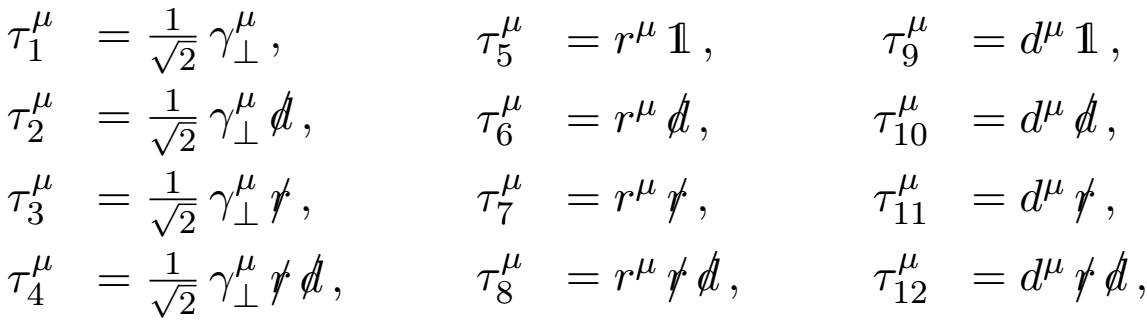
\includegraphics[width=\linewidth,  height=2.3cm]{taus.png}
  \end{figure}
\end{frame}
\endinput
